\section{Introduction}
\label{sec:intro}

Reinforcement learning against a verifier is now the standard way to improve reasoning models. Whether it teaches them
anything new is contested. \citet{yue2025doesrl} find that base models overtake their RL-trained descendants in
pass@$k$ as $k$ grows. \citet{karan2025power} approach RL's gain on a mathematics benchmark by sampling the base from a
sharpened distribution, with no training. Other work reports RL solving problems the base never solved
\citep{abdulsalam2026rewrite,liu2025prorl}. Part of the disagreement is about budgets. A base whose per-attempt
success probability on a problem is $10^{-6}$ will almost never solve it in 1,024 attempts, yet the capability is
present in a sense that matters for evaluation and safety. A capability is defined only relative to a sampling budget
\citep{li2026elicitcreate,brown2024monkeys}.

A claim that RL \emph{created} a capability therefore needs three things:
\begin{itemize}
\item a budget at which the base is judged unable, tied to what RL spent;
\item controls that receive RL's training without RL's proofs;
\item ideally, a base that never had the capability \citep{jain2023mechanistically,deeb2024unlearning}.
\end{itemize}
Pretraining interventions before RL exist. \citet{zhang2025interplay} vary a context's share of pretraining (0\%,
0.1\%, 1\%) in a 100M model and find no RL transfer below 1\%. \citet{abdulsalam2026rewrite} exclude shortcuts from
pretraining and see GRPO build them. \citet{tsilivis2025rlntp} set the share of long demonstrations exactly. We add a
narrower intervention, with the base's own rate measured. We remove a single inference composition from pretraining,
keep both of its parts, refill the data to the same size, and measure the base's rate for the composition at about a
million attempts.

We do this in a model organism small enough to allow it. It is a 9.56M-parameter transformer prover for propositional
logic, pretrained from scratch on 155,000 synthetic natural-deduction proofs. It acts through a proof-state interface,
one inference step at a time, and Lean~4 alone decides whether a proof counts. The composition we remove is the
classical reductio \sig{}: to prove a positive goal $G$, assume $\neg G$, derive a contradiction, conclude $\neg\neg G$
by negation introduction, and eliminate the double negation (\texttt{DN}, Lean's \texttt{Classical.byContradiction}).
Both rules stay in the data, used separately. We track six classical theorem families, such as excluded middle and
Peirce's law, whose \emph{strict} members can only be proved by eliminating a double negation the proof itself built.
Their 106 held-out strict theorems are never trained on. We then run expert iteration (EI) from each base: sample,
keep what Lean accepts, fine-tune, for 16 rounds (Fig.~\ref{fig:overview}).

\begin{figure}[t]
\centering
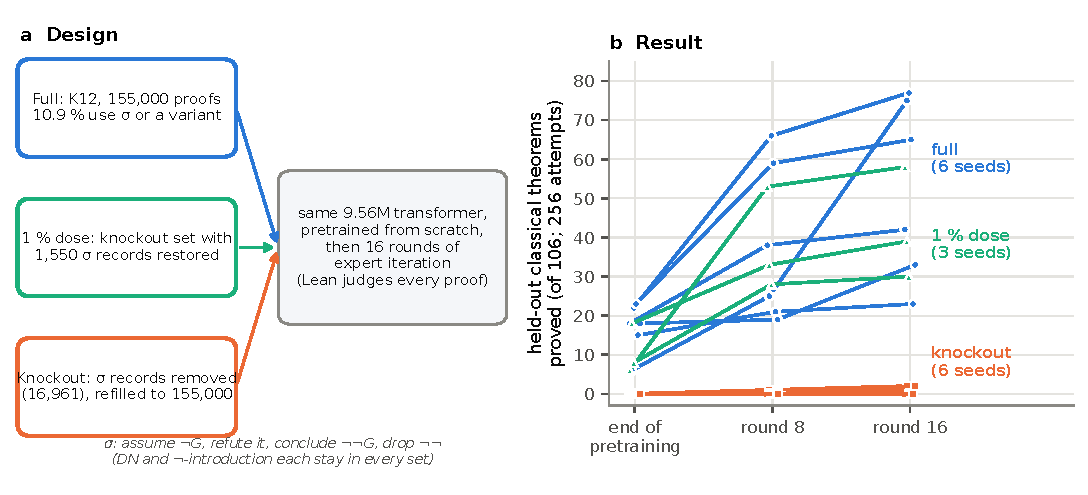
\includegraphics[width=\linewidth]{figures/fig0_overview.pdf}
\caption{\textbf{Design and result.} (a) Three pretraining sets that differ only in the classical reductio \sig{}. (b)
Held-out classical theorems proved (of 106, with 256 attempts each) at the end of pretraining and after 8 and 16 rounds
of expert iteration, one line per seed. No knockout seed acquires a classical family in 16 rounds.}
\label{fig:overview}
\end{figure}

\paragraph{Two objections, and the null model.} The first objection is that a model cannot learn what it never saw.
But the knockout bases saw both rules, and they still write \sig{}: five of six proved held-out strict theorems with it
at large sample sizes. The second objection is stronger. At the bases' measured rates, EI's 3,936 attempts per round on
the 123 strict training theorems should find at most 0.02 \sig{} proofs per round. A first success would then be
expected only after 47 rounds or more. We take this
waiting-time arithmetic as the null model and ask what happens beyond it.

\paragraph{Results.}
\begin{itemize}
\item \textbf{No knockout seed acquired a classical family in 16 rounds} (0/6, which bounds the per-seed rate below
0.39), against 6/6 full-exposure seeds. That pre-registered contrast is largely decided before RL: one family is
already acquired at the end of pretraining on 5/6 full seeds. The contrasts specific to RL were not pre-registered.
During RL, full seeds gained 8--69 held-out strict theorems and knockout seeds 0--2 (exact Mann--Whitney $p=0.0011$).
Five of six full seeds against none acquired a family during RL ($p=0.0032$; on the three seeds that shared the
knockout's hardware, 2/3 vs 0/6, $p=0.034$).
\item \textbf{One percent is enough.} Restoring \sig{} in 1\% of pretraining records restored acquisition on 3/3 seeds.
\item \textbf{Beyond the null.} The knockout ladders wrote \sig{} from round 1 on theorems that supply the double
negation, and trained on 844--4,428 such proofs. Three of six reached a strict training theorem sooner than their bases'
rates predict: 0.55 seeds expected by round 16, 3 observed, $p=0.006$ under the null. None carried the step to a
family. The ladder that went furthest, continued to 24 rounds, proved 5 of the 106 held-out theorems, more often each
round, and no more of them.
\item \textbf{Measurement.} In three earlier full-exposure runs, 51--60 theorems per run look RL-created at equal
sample counts. Only 14--21 remain when the base gets RL's compute as attempts, under every budget allocation we tried.
\end{itemize}

\paragraph{Contributions.}
\begin{enumerate}
\item \textbf{A composition knockout in pretraining} (\S\ref{sec:results}), with a dose arm and diagnostics that
separate ``absent'' from ``rare'': base rates at about $10^6$ attempts, certificates, a waiting-time null, and
likelihoods of known proofs along every RL run. It was pre-registered, with six seeds per main arm, and an analyst who
did not write the experiment's code recounted it independently.
\item \textbf{A compute-matched measurement protocol, applied end to end} (\S\ref{sec:setup}, \S\ref{sec:case}). It
gives the base a budget of attempts matched to RL's compute under several defensible allocations, so that the
``created'' set becomes a curve in the budget. It brackets each theorem's success rate between sampling bounds and a
likelihood estimate, certifies unreachability, and nets out RL-free training. It integrates budget-relative definitions
from prior work \citep{li2026elicitcreate,davidson2023retraining,wu2025invisibleleash}.
\item \textbf{An open organism}: a from-scratch prover with a sound judge, likelihoods of arbitrary proofs at every
checkpoint, and pretraining that can be edited one composition at a time. Code, data, checkpoints and per-arm compute
are public.
\end{enumerate}

\paragraph{What transfers.} The protocol and the waiting-time logic transfer to larger models; the numbers do not. The
1\% threshold, the $10^{-6}$ rates and the dynamics of EI belong to this organism, and they depend on how many training
problems need the composition. Two lessons follow, with that caveat. Failure at modest $k$ does not show absence: our
knockout bases fail at $k=256$, yet succeed at pooled rates near $10^{-6}$ per attempt, and at up to about
$5\times10^{-4}$ on a few theorems. And removing a
composition from pretraining kept this RL from acquiring it within 16 rounds, but 1\% of the data restored it.
Section~\ref{sec:discussion} discusses what other algorithms and injected demonstrations did to similar patterns in
earlier, smaller organisms.
